\section{Potential-function certificates}
\label{sec:potential}

The potential method follows Erd\H{o}s and Selfridge's hypergraph criterion
and its biased-game form developed by Beck \cite{erdos-selfridge-1973,beck-2008}.
Here it supplies sufficient blocking certificates for selected Hexo windows.
Window births prevent the direct global invariant from giving an unrestricted
forever theorem.

\subsection{Potential and the round inequality}

The potential counts only attacker-touched windows that remain available to
the attacker.

\begin{definition}[Residual potential; companion D3 and D4]
\label{def:ES-D3}
Let $F$ be a finite labelled family of attacker target windows.  At a position
$P$, write $A$ and $D$ for the sets of cells occupied by attacker and defender
stones, respectively, and put
\[
  \mathcal L_F(P)=\{W\in F:W\cap D=\varnothing\},
  \qquad E_P(W)=W\setminus A,
\]
and set
\[
  \lambda=\sqrt3,
  \qquad
  \Psi_F(P)=\sum_{W\in\mathcal L_F(P)}\lambda^{-|E_P(W)|}.
\]
The dynamic potential is
\[
  \Phi(P)=
  \sum_{\substack{W:\,W\cap A\ne\varnothing\\W\cap D=\varnothing}}
       \lambda^{-e_P(W)},
  \qquad e_P(W)=|W\setminus A|.
\]
Thus $\Phi$ includes exactly the attacker-touched alive windows.  All-empty
windows are excluded: including them would add $\lambda^{-6}=1/27$ for
infinitely many windows and make the sum diverge.

For an empty cell $x$, define its fixed-family danger by
\[
  d_F(x;P)=
  \sum_{\substack{W\in\mathcal L_F(P)\\x\in E_P(W)}}
       \lambda^{-|E_P(W)|}.
\]
Sequential greedy defense recomputes this danger before each of the defender's
two placements and chooses a maximum-danger empty cell, using fixed
deterministic tie-breaking.  When every scored danger is zero, the filler
chooses an occupied cell of maximum $q$, breaking ties by maximum $r$, and
places at its neighbor one step in the positive $Q$ direction.
\end{definition}

The value $\lambda=\sqrt3$ is the largest, and hence optimal, base supported
by the two-defender, two-attacker round calculation.

\begin{lemma}[One full fixed-family round; companion L5]
\label{lem:ES-L5}
Let the defender make two sequential greedy placements in a fixed residual
family, followed by at most two attacker placements.  Assume either that all
positive-danger cells are legal or that every surviving label is
attacker-alive.  The fixed-family potential at the next defender epoch is no
larger than at the preceding defender epoch.
\end{lemma}

\begin{proof}
Let $\delta_1$ and $\delta_2$ be the exact reductions made by the two greedy
defender placements.  After both placements, let
\[
  S=\max_x d_F(x)
\]
over the remaining empty cells.  Deleting edges never increases a cell's
danger.  The first and second greedy maxima are therefore both at least $S$,
so
\begin{equation}
  \delta_1+\delta_2\ge2S. \label{eq:ES-defender}
\end{equation}
An attacker placement at $x$ multiplies by $\lambda$ the weight of each
residual edge containing $x$, and hence increases the potential by exactly
$(\lambda-1)d_F(x)$.  After one attacker placement every remaining danger is
at most $\lambda S$.  The two attacker placements therefore increase the
potential by at most
\begin{equation}
  (\lambda-1)(1+\lambda)S
  =(\lambda^2-1)S=2S. \label{eq:ES-attacker}
\end{equation}
Equations \eqref{eq:ES-defender}--\eqref{eq:ES-attacker} show that the full
round change is nonpositive.  If play stops after the first attacker
placement, omitting the second nonnegative increase only strengthens the
inequality up to that placement.
\end{proof}

Base $2$ does not support the claimed blocking threshold.  Take three target
windows so far apart that no length-six window intersects two of them, and put
four attacker stones in each target.  Each target then has weight $2^{-2}$,
so the sum is $3/4<1$.  The defender can kill at most two separated targets
in one turn.  The attacker fills the two empties of the survivor and wins.

\subsection{Certificates and their boundary}

The fixed-family theorem applies only at the start of a full defender turn.

\begin{theorem}[Fixed-family Hexo blocking; companion Theorem 1]
\label{thm:ES-T1}
Let $P_0$ be a nonterminal defender-\textup{FirstStone} position, and let $F$
be any finite fixed family of windows that are attacker-alive at $P_0$.  If
\[
  \Psi_F(P_0)<1,
\]
then sequential greedy defense prevents the attacker from ever completing a
window in $F$.
\end{theorem}

\begin{proof}[Proof in the companion]
The round inequality keeps $\Psi_F<1$ at every defender epoch and through the
relevant prefixes of the following attacker pair, whereas a completed target
has a term of weight $1$.  The full-turn premise is used for both greedy
reductions.  With only one defender placement remaining, two separated
count-$4$ targets have potential $2/3<1$, but one survives and is completed.
The condition is sufficient only; one defender stone may kill as many as 18
windows, so necessity is false.  The complete proof is in
\cite{hexobot-companions}.
\end{proof}

For the dynamic family, newly touched windows must be enrolled after they are
born.

\begin{definition}[Defender epochs and birth mass; companion D5]
\label{def:ES-D5}
Let $P_t$ be the position at the start of the defender's $t$th full turn.
During the following attacker pair, or its prefix before a terminal placement,
let $N_t$ consist of the windows that were stone-free at $P_t$, were not hit by
the intervening defender pair, and first became attacker-alive during that
attacker pair.  For $W\in N_t$, let $a_t(W)\in\{1,2\}$ be the number of stones
from that pair in $W$ at the end of the pair or terminal prefix.  Its exact
birth mass is
\[
  C_t=\sum_{W\in N_t}\lambda^{-(6-a_t(W))}.
\]
After a terminal play, all later source terms are zero.
\end{definition}

The potential below one does certify the next complete attack cycle.

\begin{theorem}[Global one-cycle certificate; companion Theorem 2]
\label{thm:ES-T2}
If the defender is at \textup{FirstStone} and the current dynamic potential
satisfies $\Phi(P_t)<1$, then two sequential touched-window greedy placements
prevent the attacker from winning during the immediately following
two-placement turn.
\end{theorem}

\begin{proof}[Proof in the companion]
\Cref{thm:ES-T1} blocks every currently alive window, including a completion
on the first attacker placement.  A different potential winning window either
already has a permanent defender stone or was stone-free at $P_t$ and cannot
receive six stones in one attacker pair.  This is not a forever certificate,
because births may put $\Phi(P_{t+1})$ above $1$.  The complete proof is in
\cite{hexobot-companions}.
\end{proof}

A forever statement requires a bound that is uniform over attacker
strategies, not a source sum observed along one path.

\begin{theorem}[Cumulative-birth forever certificate; companion Theorem 3]
\label{thm:ES-T3}
Fix the tie-breaking and filler policy in \cref{def:ES-D3}, and use sequential
touched-window greedy defense from $P_0$.  Suppose a uniform constant
$B_\infty$ satisfies
\[
  \sup_{\tau}\sum_{t=0}^{\infty}C_t(\tau)\le B_\infty,
  \qquad \Phi(P_0)+B_\infty<1,
\]
where the supremum is over every legal attacker strategy $\tau$.  Then the
defender prevents the attacker from ever completing a window.  More generally,
if $B_T$ is a uniform upper bound satisfying
\[
  \sup_{\tau}\sum_{t=0}^{T-1}C_t(\tau)\le B_T,
  \qquad \Phi(P_0)+B_T<1,
\]
then the first $T$ attacker pairs, indexed $0,\ldots,T-1$, are certified.
\end{theorem}

\begin{proof}[Proof in the companion]
The dynamic recurrence
$\Phi(P_{t+1})\le\Phi(P_t)+C_t$ and induction keep the potential below one
before each certified pair, so \cref{thm:ES-T2} applies repeatedly.  The
supremum is used to make the same argument against every attacker strategy;
a pathwise observed value of $\sum_t C_t$ has the wrong quantifier and is not
a certificate.  The complete proof is in \cite{hexobot-companions}.
\end{proof}

Finite confinement supplies a computable reservoir of virgin windows.

\begin{definition}[Finite-region targets; companion D6]
\label{def:ES-D6}
Fix a defender epoch $P_0$ and a finite set $R$ of cells empty at $P_0$.
Assume every future attacker placement is confined to $R$.  Define
\[
\begin{aligned}
  \mathcal A_R&=\{W:W\cap D_0=\varnothing,\ W\cap A_0\ne\varnothing,
                         \ W\setminus A_0\subseteq R\},\\
  \mathcal V_R&=\{W:W\textup{ is stone-free at }P_0,\ W\subseteq R\},
  \qquad N_R=|\mathcal V_R|,
\end{aligned}
\]
and
\[
  \Phi_R(P_0)=\sum_{W\in\mathcal A_R}\lambda^{-e_{P_0}(W)}.
\]
Region-target greedy scores only currently attacker-alive members of the fixed
target family $\mathcal H_R=\mathcal A_R\cup\mathcal V_R$.
\end{definition}

\begin{definition}[Virgin activation reserve; companion D7 and Lemma 9]
\label{def:ES-D7}
For a matching $M$ of pairwise vertex-disjoint two-cell subsets of $R$, let
\[
  q(M)=|\{W\in\mathcal V_R:\textup{ some }\{x,y\}\in M
                                      \textup{ satisfies }x,y\in W\}|,
\]
and put
\[
  P_R=\max_M q(M),
  \qquad
  B_R^*=N_R\lambda^{-5}+P_R(\lambda^{-4}-\lambda^{-5}).
\]
For certification, $P_R$ must be evaluated exactly or replaced by a proved
upper bound, such as
$P_R\le\min\{N_R,5\lfloor|R|/2\rfloor\}$.  An exhibited matching gives only a
lower bound and is unsafe here.  The coarser reserve is $B_R^*\le N_R/9$.
\end{definition}

\begin{theorem}[Finite-region forever theorem; companion Theorem 4]
\label{thm:ES-T4}
If the attacker is forever confined to the finite region $R$ and
\[
  \Phi_R(P_0)+B_R^*<1,
\]
then region-target greedy defense prevents the attacker from ever winning.
The weaker sufficient condition
\[
  \Phi_R(P_0)+\frac{N_R}{9}<1
\]
has the same conclusion.  Every positive-reduction defender placement made by
this strategy is an empty cell of a currently attacker-alive member of
$\mathcal H_R$ and is legal.  The confinement is on the attacker; defender
fillers may lie outside $R$.
\end{theorem}

\begin{proof}[Proof in the companion]
Delayed enrollment gives the fixed-target recurrence, while the matching
reserve charges each virgin window once and charges the larger two-stone birth
weight to at most $P_R$ windows.  Every window completable under confinement
belongs to $\mathcal A_R$ or $\mathcal V_R$.  The confinement premise must
come from a separate certificate; the theorem does not establish it.  The
complete proof is in \cite{hexobot-companions}.
\end{proof}

\begin{figure}[tbp]
  \centering
  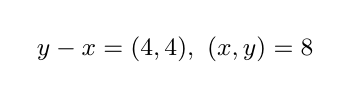
\begin{tikzpicture}
    \begin{scope}[xshift=-4.0cm,scale=.34]
      \HexPatch{-2/0,-1/0,0/0,1/0,2/0,3/0,
        0/-2,0/-1,0/1,0/2,0/3,
        -2/2,-1/1,1/-1,2/-2,3/-3}
      \HexWindow[fill=black!7,draw=none]{-2}{0}{1}{0}
      \HexWindow[fill=black!11,draw=none]{0}{-2}{0}{1}
      \HexWindow[fill=black!15,draw=none]{-2}{2}{1}{-1}
      \HexAttacker{0}{0}
    \end{scope}
    \begin{scope}[xshift=4.0cm,scale=.34]
      \HexPatch{-2/0,-1/0,0/0,1/0,2/0,3/0,
        0/-2,0/-1,0/1,0/2,0/3,
        -2/2,-1/1,1/-1,2/-2,3/-3}
      \HexWindow[fill=black!7,draw=none]{-2}{0}{1}{0}
      \HexWindow[fill=black!11,draw=none]{0}{-2}{0}{1}
      \HexWindow[fill=black!15,draw=none]{-2}{2}{1}{-1}
      \HexAttacker{0}{0}
    \end{scope}
    \draw[<->,densely dashed] (-1.7,0) -- node[fill=white,font=\small]
      {$y-x=(4,4),\ \dist(x,y)=8$} (1.7,0);
  \end{tikzpicture}
  \caption{Counterexample 1, schematically.  The two attacker placements are
  at hex distance $8$, off all three axes, and have disjoint clean window
  stars.  Together they enroll 36
  one-stone windows, and the potential jumps from $0$ to
  $36\lambda^{-5}=4/\sqrt3>1$.  Three of the 18 windows through each new
  stone are shaded.}
  \label{fig:es-birth}
\end{figure}

\subsection{Practical domain and open boundary}

The exact node test can be performed without floating-point arithmetic.

\begin{corollary}[Integer-only threshold check; companion Corollary 2]
\label{cor:ES-C2}
At a nonterminal position, for $s=1,\ldots,5$, let $n_s$ be the number of
currently attacker-alive windows with exactly $s$ attacker stones.  Put
\[
  a=n_1+3n_3+9n_5,
  \qquad b=n_2+3n_4.
\]
Then
\[
  \Phi<1
  \quad\Longleftrightarrow\quad
  b\le8,\qquad a^2<3(9-b)^2.
\]
\end{corollary}

Indeed, $\Phi<1$ is $a+\sqrt3b<9\sqrt3$.  The right side of
$a<\sqrt3(9-b)$ must be positive, giving $b\le8$, after which squaring is
equivalent.  This check costs $O(\#\text{touched windows})$, not
$O(\#\text{threats})$.

If $I=\sum_{s=1}^5s n_s$ is the number of attacker-stone/alive-window
incidences, then $\Phi\ge I/18$.  Thus $\Phi<1$ forces $I\le17$.  With $N_A$
attacker stones, all but at most 17 of the $18N_A$ incidences must already lie
in defender-killed windows.  The practical domain is therefore a heavily
blocked, endgame-like region rather than a general middlegame.

The raw global claim that $\Phi<1$ blocks the unrestricted infinite game
forever remains open.  Counterexample 1 starts with $\Phi=0$ and, after the
fixed zero-danger fillers, uses two far placements to birth 36 one-stone
windows, producing $4/\sqrt3>1$ as shown in \cref{fig:es-birth}.  Requiring
that no current attacker window have at most two empties does not repair the
invariant, because the condition holds vacuously at $\Phi=0$ before the same
births.  Replacing $\Phi<1$ by $\Phi\le1$ also fails: three separated count-$4$
targets have total potential $1$, the defender kills at most two, and the
attacker completes the survivor.  These are failures of the proposed
potential certificates, not proofs that the attacker wins every corresponding
unrestricted game.  The $\Phi=1$ example is a static blanket-game
construction; it is not asserted to be a material-balanced reachable engine
position and does not prove sharpness after restriction to reachable nodes.

Every positive-reduction greedy placement lies in an attacker-touched alive
window and therefore inside the relevance closure of \cref{sec:computable-zones}.
If no monitored window remains, one or both placements of a defender turn may
instead be arbitrary legal fillers.  The certified strategy must permit these
fillers.  Their presence does not affect the dismissal soundness theorem; it
only constrains the potential-certified strategy.
